\documentclass{article}\usepackage[]{graphicx}\usepackage[]{color}
%% maxwidth is the original width if it is less than linewidth
%% otherwise use linewidth (to make sure the graphics do not exceed the margin)
\makeatletter
\def\maxwidth{ %
  \ifdim\Gin@nat@width>\linewidth
    \linewidth
  \else
    \Gin@nat@width
  \fi
}
\makeatother

\definecolor{fgcolor}{rgb}{0.345, 0.345, 0.345}
\newcommand{\hlnum}[1]{\textcolor[rgb]{0.686,0.059,0.569}{#1}}%
\newcommand{\hlstr}[1]{\textcolor[rgb]{0.192,0.494,0.8}{#1}}%
\newcommand{\hlcom}[1]{\textcolor[rgb]{0.678,0.584,0.686}{\textit{#1}}}%
\newcommand{\hlopt}[1]{\textcolor[rgb]{0,0,0}{#1}}%
\newcommand{\hlstd}[1]{\textcolor[rgb]{0.345,0.345,0.345}{#1}}%
\newcommand{\hlkwa}[1]{\textcolor[rgb]{0.161,0.373,0.58}{\textbf{#1}}}%
\newcommand{\hlkwb}[1]{\textcolor[rgb]{0.69,0.353,0.396}{#1}}%
\newcommand{\hlkwc}[1]{\textcolor[rgb]{0.333,0.667,0.333}{#1}}%
\newcommand{\hlkwd}[1]{\textcolor[rgb]{0.737,0.353,0.396}{\textbf{#1}}}%

\usepackage{framed}
\makeatletter
\newenvironment{kframe}{%
 \def\at@end@of@kframe{}%
 \ifinner\ifhmode%
  \def\at@end@of@kframe{\end{minipage}}%
  \begin{minipage}{\columnwidth}%
 \fi\fi%
 \def\FrameCommand##1{\hskip\@totalleftmargin \hskip-\fboxsep
 \colorbox{shadecolor}{##1}\hskip-\fboxsep
     % There is no \\@totalrightmargin, so:
     \hskip-\linewidth \hskip-\@totalleftmargin \hskip\columnwidth}%
 \MakeFramed {\advance\hsize-\width
   \@totalleftmargin\z@ \linewidth\hsize
   \@setminipage}}%
 {\par\unskip\endMakeFramed%
 \at@end@of@kframe}
\makeatother

\definecolor{shadecolor}{rgb}{.97, .97, .97}
\definecolor{messagecolor}{rgb}{0, 0, 0}
\definecolor{warningcolor}{rgb}{1, 0, 1}
\definecolor{errorcolor}{rgb}{1, 0, 0}
\newenvironment{knitrout}{}{} % an empty environment to be redefined in TeX

\usepackage{alltt}
\usepackage[sc]{mathpazo}
\renewcommand{\sfdefault}{lmss}
\renewcommand{\ttdefault}{lmtt}
\usepackage[T1]{fontenc}
\usepackage{geometry}
\geometry{verbose,tmargin=2.5cm,bmargin=2.5cm,lmargin=2.5cm,rmargin=2.5cm}
\setcounter{secnumdepth}{2}
\setcounter{tocdepth}{2}
\usepackage[unicode=true,pdfusetitle,
 bookmarks=true,bookmarksnumbered=true,bookmarksopen=true,bookmarksopenlevel=2,
 breaklinks=false,pdfborder={0 0 1},backref=false,colorlinks=false]
 {hyperref}
\hypersetup{
 pdfstartview={XYZ null null 1}}

\makeatletter
%%%%%%%%%%%%%%%%%%%%%%%%%%%%%% User specified LaTeX commands.
\renewcommand{\textfraction}{0.05}
\renewcommand{\topfraction}{0.8}
\renewcommand{\bottomfraction}{0.8}
\renewcommand{\floatpagefraction}{0.75}

\makeatother
\IfFileExists{upquote.sty}{\usepackage{upquote}}{}
\begin{document}








The results below are generated from an R script.

\begin{knitrout}
\definecolor{shadecolor}{rgb}{0.969, 0.969, 0.969}\color{fgcolor}\begin{kframe}
\begin{alltt}
\hlstd{nom.col}\hlkwb{<-} \hlkwd{c}\hlstd{(}\hlstr{"dossier"}\hlstd{,}\hlstr{"Libelle"}\hlstd{,}\hlstr{"Date"}\hlstd{,}\hlstr{"Age_en_clair"}\hlstd{,}\hlstr{"Age_en_annees"}\hlstd{,}\hlstr{"Age_en_jours"}\hlstd{,}\hlstr{"Nombre"}\hlstd{,}\hlstr{"Mission"}\hlstd{,}\hlstr{"Moyen"}\hlstd{,}\hlstr{"Commune"}\hlstd{,}\hlstr{"Etablissement_intervention"}\hlstd{,}\hlstr{"Sexe"}\hlstd{,}\hlstr{"Devenir"}\hlstd{,}\hlstr{"Moyen_evac"}\hlstd{,}\hlstr{"Commune_destination"}\hlstd{,}\hlstr{"Etablissement_destination"}\hlstd{,}\hlstr{"Service_destination"}\hlstd{)}

\hlstd{path} \hlkwb{<-} \hlstr{"../"}

\hlstd{file} \hlkwb{<-} \hlkwd{paste0}\hlstd{(path,} \hlstr{"data/activite_helico_2013.csv"}\hlstd{)}
\hlstd{he} \hlkwb{<-} \hlkwd{read.csv}\hlstd{(file)}
\end{alltt}


{\ttfamily\noindent\color{warningcolor}{\#\# Warning in file(file, "{}rt"{}): impossible d'ouvrir le fichier '../data/activite\_helico\_2013.csv' : No such file or directory}}

{\ttfamily\noindent\bfseries\color{errorcolor}{\#\# Error in file(file, "{}rt"{}): impossible d'ouvrir la connexion}}\begin{alltt}
\hlkwd{colnames}\hlstd{(he)} \hlkwb{<-} \hlstd{nom.col}
\end{alltt}


{\ttfamily\noindent\bfseries\color{errorcolor}{\#\# Error in `colnames<-`(`*tmp*`, value = c("{}dossier"{}, "{}Libelle"{}, "{}Date"{}, : attempt to set 'colnames' on an object with less than two dimensions}}\begin{alltt}
\hlstd{h2} \hlkwb{<-} \hlstd{he[}\hlopt{!}\hlkwd{duplicated}\hlstd{(he}\hlopt{$}\hlstd{dossier),]}
\end{alltt}


{\ttfamily\noindent\bfseries\color{errorcolor}{\#\# Error in he\$dossier: \$ operator is invalid for atomic vectors}}\begin{alltt}
\hlstd{H2013} \hlkwb{<-} \hlstd{h2}

\hlstd{file} \hlkwb{<-} \hlkwd{paste0}\hlstd{(path,} \hlstr{"data/activite_helico_2012.csv"}\hlstd{)}
\hlstd{he} \hlkwb{<-} \hlkwd{read.csv}\hlstd{(file)}
\end{alltt}


{\ttfamily\noindent\color{warningcolor}{\#\# Warning in file(file, "{}rt"{}): impossible d'ouvrir le fichier '../data/activite\_helico\_2012.csv' : No such file or directory}}

{\ttfamily\noindent\bfseries\color{errorcolor}{\#\# Error in file(file, "{}rt"{}): impossible d'ouvrir la connexion}}\begin{alltt}
\hlkwd{colnames}\hlstd{(he)} \hlkwb{<-} \hlstd{nom.col}
\end{alltt}


{\ttfamily\noindent\bfseries\color{errorcolor}{\#\# Error in `colnames<-`(`*tmp*`, value = c("{}dossier"{}, "{}Libelle"{}, "{}Date"{}, : attempt to set 'colnames' on an object with less than two dimensions}}\begin{alltt}
\hlstd{h2} \hlkwb{<-} \hlstd{he[}\hlopt{!}\hlkwd{duplicated}\hlstd{(he}\hlopt{$}\hlstd{dossier),]}
\end{alltt}


{\ttfamily\noindent\bfseries\color{errorcolor}{\#\# Error in he\$dossier: \$ operator is invalid for atomic vectors}}\begin{alltt}
\hlstd{H2012} \hlkwb{<-} \hlstd{h2}
\end{alltt}
\end{kframe}
\end{knitrout}
\begin{knitrout}
\definecolor{shadecolor}{rgb}{0.969, 0.969, 0.969}\color{fgcolor}\begin{kframe}
\begin{alltt}
\hlstd{h2} \hlkwb{<-} \hlkwd{rbind}\hlstd{(H2012, H2013)}
\end{alltt}
\end{kframe}
\end{knitrout}
\begin{knitrout}
\definecolor{shadecolor}{rgb}{0.969, 0.969, 0.969}\color{fgcolor}\begin{kframe}
\begin{alltt}
\hlstd{h2}\hlopt{$}\hlstd{Jour} \hlkwb{<-} \hlkwd{as.Date}\hlstd{(}\hlkwd{substr}\hlstd{(h2}\hlopt{$}\hlstd{Date,} \hlnum{1}\hlstd{,} \hlnum{10}\hlstd{),} \hlstr{"%d/%m/%Y"}\hlstd{)}
\hlstd{h2}\hlopt{$}\hlstd{heure} \hlkwb{<-} \hlkwd{substr}\hlstd{(h2}\hlopt{$}\hlstd{Date,} \hlnum{12}\hlstd{,} \hlnum{17}\hlstd{)} \hlcom{# heures/minutes}

\hlstd{h2}\hlopt{$}\hlstd{he} \hlkwb{<-} \hlkwd{substr}\hlstd{(h2}\hlopt{$}\hlstd{Date,} \hlnum{12}\hlstd{,} \hlnum{13}\hlstd{)} \hlcom{# heures pleines}
\hlkwd{barplot}\hlstd{(}\hlkwd{table}\hlstd{(}\hlkwd{as.factor}\hlstd{(h2}\hlopt{$}\hlstd{he)))} \hlcom{# primaires et secondaires}
\end{alltt}
\end{kframe}

{\centering 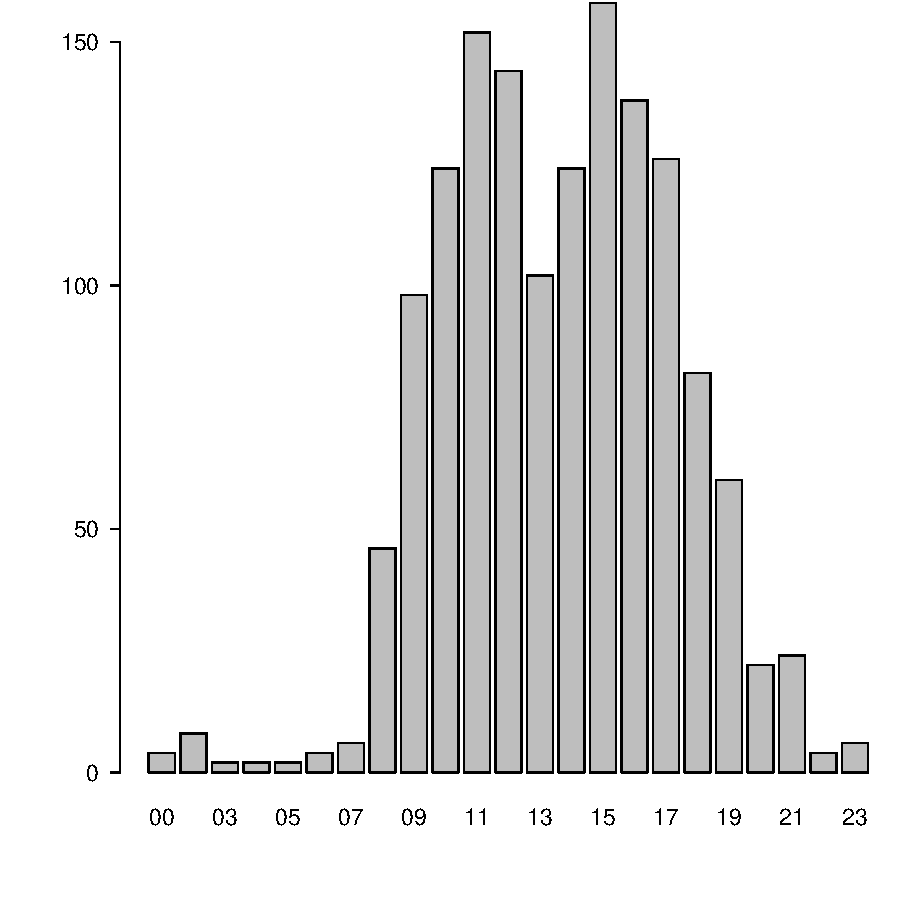
\includegraphics[width=.6\linewidth]{figure/helico-Rnwunnamed-chunk-3-1} 

}


\begin{kframe}\begin{alltt}
\hlkwd{barplot}\hlstd{(}\hlkwd{table}\hlstd{(h2}\hlopt{$}\hlstd{Mission,} \hlkwd{as.factor}\hlstd{(h2}\hlopt{$}\hlstd{he)))} \hlcom{# primaireset secondaires séparées}
\end{alltt}
\end{kframe}

{\centering 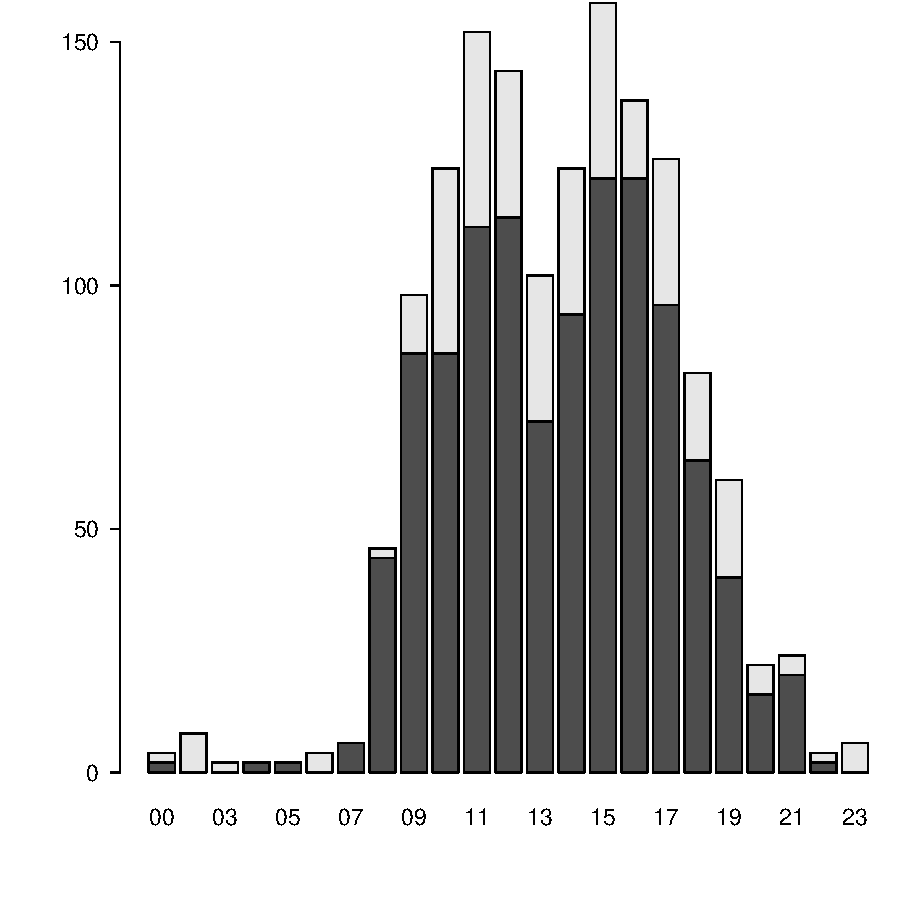
\includegraphics[width=.6\linewidth]{figure/helico-Rnwunnamed-chunk-3-2} 

}


\begin{kframe}\begin{alltt}
\hlkwd{barplot}\hlstd{(}\hlkwd{table}\hlstd{(h2}\hlopt{$}\hlstd{Mission,} \hlkwd{as.factor}\hlstd{(h2}\hlopt{$}\hlstd{he)),} \hlkwc{beside} \hlstd{=} \hlnum{TRUE}\hlstd{)}
\end{alltt}
\end{kframe}

{\centering 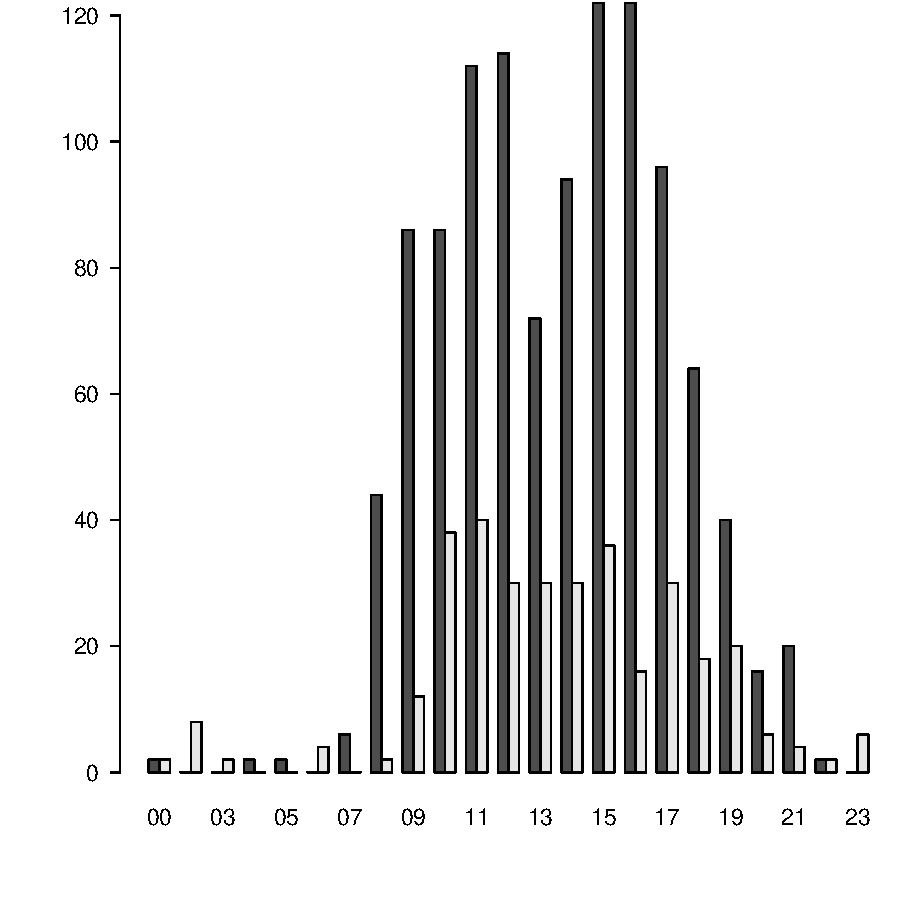
\includegraphics[width=.6\linewidth]{figure/helico-Rnwunnamed-chunk-3-3} 

}



\end{knitrout}
\begin{knitrout}
\definecolor{shadecolor}{rgb}{0.969, 0.969, 0.969}\color{fgcolor}\begin{kframe}
\begin{alltt}
\hlstd{n.missions} \hlkwb{<-} \hlkwd{nrow}\hlstd{(h2)}
\hlstd{n.missions.jour} \hlkwb{<-} \hlstd{n.missions}\hlopt{/}\hlnum{365}

\hlkwd{table}\hlstd{(h2}\hlopt{$}\hlstd{Mission)}
\end{alltt}
\begin{verbatim}
## 
##  Primaire Transfert 
##      1102       336
\end{verbatim}
\begin{alltt}
\hlkwd{prop.table}\hlstd{(}\hlkwd{table}\hlstd{(h2}\hlopt{$}\hlstd{Mission))}
\end{alltt}
\begin{verbatim}
## 
##  Primaire Transfert 
## 0.7663421 0.2336579
\end{verbatim}
\begin{alltt}
\hlkwd{table}\hlstd{(h2}\hlopt{$}\hlstd{Sexe)}
\end{alltt}
\begin{verbatim}
## 
##  Femmes  Hommes Inconnu 
##     498     908      32
\end{verbatim}
\begin{alltt}
\hlkwd{table}\hlstd{(h2}\hlopt{$}\hlstd{Devenir)}
\end{alltt}
\begin{verbatim}
## < table of extent 0 >
\end{verbatim}
\begin{alltt}
\hlkwd{table}\hlstd{(h2}\hlopt{$}\hlstd{Devenir, h2}\hlopt{$}\hlstd{Mission)}
\end{alltt}


{\ttfamily\noindent\bfseries\color{errorcolor}{\#\# Error in table(h2\$Devenir, h2\$Mission): all arguments must have the same length}}\begin{alltt}
\hlkwd{table}\hlstd{(h2}\hlopt{$}\hlstd{Commune_destination)}
\end{alltt}
\begin{verbatim}
## 
##                                  ALLEMAGNE B6                 AUTRES 
##                    148                      2                      6 
##               BESANCON                 COLMAR                FORBACH 
##                      2                     86                      4 
##     FREYMING MERLEBACH               FRIBOURG               HAGUENAU 
##                      2                      2                    188 
## ILLKIRCH GRAFFENSTADEN  LUDWIGSHAFEN AM RHEIN                   LYON 
##                      2                      6                      2 
##                   METZ            MONTBELIARD               MULHOUSE 
##                     18                      2                     26 
##                  NANCY                  PARIS                  REIMS 
##                      8                      4                      0 
##             REMIREMONT            SAINT AVOLD   SAINT DIE DES VOSGES 
##                      2                      2                      6 
##             SARREBOURG          SARREGUEMINES                SAVERNE 
##                     10                     10                     76 
##              SCHIRMECK               SELESTAT             STRASBOURG 
##                     10                     58                    738 
##   VANDOEUVRE LES NANCY                 VERDUN            WISSEMBOURG 
##                      4                      2                     12
\end{verbatim}
\begin{alltt}
\hlkwd{table}\hlstd{(h2}\hlopt{$}\hlstd{Commune_destination, h2}\hlopt{$}\hlstd{Mission)}
\end{alltt}
\begin{verbatim}
##                         
##                          Primaire Transfert
##                               146         2
##   ALLEMAGNE B6                  2         0
##   AUTRES                        4         2
##   BESANCON                      0         2
##   COLMAR                       60        26
##   FORBACH                       0         4
##   FREYMING MERLEBACH            0         2
##   FRIBOURG                      2         0
##   HAGUENAU                    176        12
##   ILLKIRCH GRAFFENSTADEN        0         2
##   LUDWIGSHAFEN AM RHEIN         2         4
##   LYON                          0         2
##   METZ                          8        10
##   MONTBELIARD                   0         2
##   MULHOUSE                      4        22
##   NANCY                         4         4
##   PARIS                         0         4
##   REIMS                         0         0
##   REMIREMONT                    2         0
##   SAINT AVOLD                   0         2
##   SAINT DIE DES VOSGES          6         0
##   SARREBOURG                    4         6
##   SARREGUEMINES                10         0
##   SAVERNE                      68         8
##   SCHIRMECK                    10         0
##   SELESTAT                     52         6
##   STRASBOURG                  530       208
##   VANDOEUVRE LES NANCY          2         2
##   VERDUN                        0         2
##   WISSEMBOURG                  10         2
\end{verbatim}
\end{kframe}
\end{knitrout}
\begin{knitrout}
\definecolor{shadecolor}{rgb}{0.969, 0.969, 0.969}\color{fgcolor}\begin{kframe}
\begin{alltt}
\hlkwd{summary}\hlstd{(h2}\hlopt{$}\hlstd{Age_en_annees)}
\end{alltt}
\begin{verbatim}
##    Min. 1st Qu.  Median    Mean 3rd Qu.    Max. 
##    0.00   35.00   55.00   52.19   73.00   99.00
\end{verbatim}
\begin{alltt}
\hlkwd{hist}\hlstd{(h2}\hlopt{$}\hlstd{Age_en_annees)}
\end{alltt}
\end{kframe}

{\centering 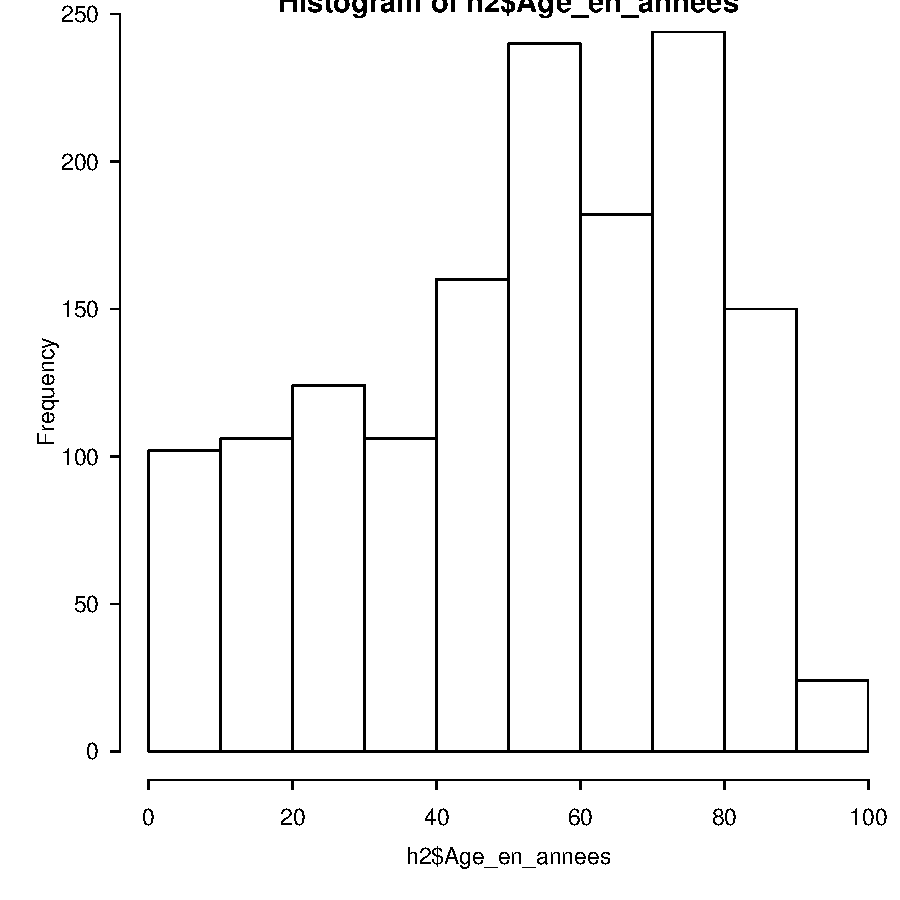
\includegraphics[width=.6\linewidth]{figure/helico-Rnwunnamed-chunk-5-1} 

}


\begin{kframe}\begin{alltt}
\hlkwd{boxplot}\hlstd{(h2}\hlopt{$}\hlstd{Age_en_annees} \hlopt{~} \hlstd{h2}\hlopt{$}\hlstd{Sexe)}
\end{alltt}
\end{kframe}

{\centering 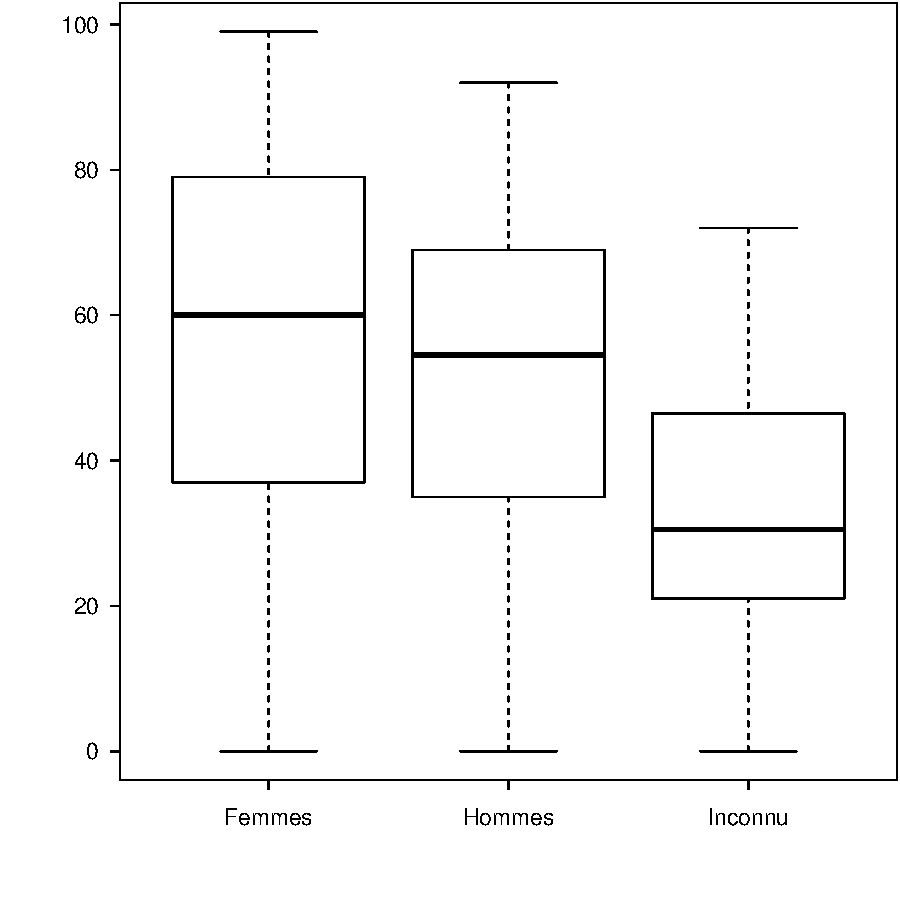
\includegraphics[width=.6\linewidth]{figure/helico-Rnwunnamed-chunk-5-2} 

}



\end{knitrout}
\begin{knitrout}
\definecolor{shadecolor}{rgb}{0.969, 0.969, 0.969}\color{fgcolor}\begin{kframe}
\begin{alltt}
\hlkwd{table}\hlstd{(h2}\hlopt{$}\hlstd{Commune[h2}\hlopt{$}\hlstd{Mission} \hlopt{==} \hlstr{"Primaire"}\hlstd{])}
\end{alltt}
\begin{verbatim}
## 
##                                   ADAMSWILLER            ALLENWILLER 
##                      2                      2                      2 
##                 ANDLAU             BAERENDORF          BALLON ALSACE 
##                      4                      2                      0 
##                   BARR             BASSEMBERG               BEINHEIM 
##                      6                      2                      4 
##                BELFORT             BELLEFOSSE                BELMONT 
##                      2                      8                      6 
##                BENFELD                   BERG         BERNARDSWILLER 
##                      8                      2                      2 
##             BETSCHDORF             BIBLISHEIM            BINDERNHEIM 
##                      4                      2                      2 
##             BIRKENWALD          BISCHOFFSHEIM   BISCHTROFF SUR SARRE 
##                      2                      4                      4 
##            BISCHWILLER                BISSERT                 BITCHE 
##                     16                      2                      2 
##           BITSCHHOFFEN              BLAESHEIM                BOERSCH 
##                      4                      2                      4 
##              BOOFZHEIM              BOURGHEIM             BOUXWILLER 
##                      8                      2                     12 
##            BREITENBACH                BRUMATH                   BUHL 
##                      6                      2                      2 
##                   BUST              BUSWILLER              CHATENOIS 
##                      2                      2                      2 
##              CLEEBOURG               CLIMBACH     COL DE LA SCHLUCHT 
##                      4                      2                      2 
##                 COLMAR        COLROY LA ROCHE                   DABO 
##                      0                      4                      2 
##             DAHLENHEIM                DAMBACH       DAMBACH LA VILLE 
##                      2                      2                      2 
##              DAUENDORF              DEHLINGEN             DETTWILLER 
##                      4                      2                      4 
##            DIEBOLSHEIM             DIEDENDORF     DIEFFENBACH AU VAL 
##                      2                      2                      2 
##    DIEFFENBACH AU VAL  DIEFFENBACH LES WOERTH            DIEMERINGEN 
##                      2                      2                      8 
##              DINGSHEIM    DINSHEIM SUR BRUCHE              DOMFESSEL 
##                      2                      2                      2 
##             DORLISHEIM           DRACHENBRONN              DRULINGEN 
##                      4                      2                      8 
##             DRUSENHEIM            DUNTZENHEIM             DUPPIGHEIM 
##                      8                      2                      4 
##              DURNINGEN            DUTTLENHEIM              EBERSHEIM 
##                      2                      6                      2 
##            EBERSVILLER          ECKARTSWILLER            ECKBOLSHEIM 
##                      2                      4                      2 
##            ECKWERSHEIM                 EPINAL             ERGERSHEIM 
##                      2                      0                      2 
## ERNOLSHEIM LES SAVERNE  ERNOLSHEIM SUR BRUCHE                ERSTEIN 
##                      2                      2                     12 
##               ESCHBACH              ESCHBOURG                 FOUCHY 
##                      2                      2                      2 
##                 FOUDAY           FRIEDOLSHEIM             FURDENHEIM 
##                      6                      2                      2 
##              GAMBSHEIM              GERSTHEIM            GEUDERTHEIM 
##                      4                      6                      2 
##              GOERSDORF               GOLDBACH             GOTTESHEIM 
##                      8                      2                      2 
##             GOUGENHEIM          GRANDFONTAINE           GRENDELBRUCH 
##                      2                      2                     10 
##            GRESSWILLER                  GRIES                 HAEGEN 
##                      2                      8                      4 
##               HAGUENAU            HARSKIRCHEN           HEILIGENBERG 
##                     12                      2                      6 
##                 HEMING            HERBITZHEIM              HESCHBACH 
##                      2                      8                      2 
##             HESSENHEIM             HIRSCHLAND             HOCHFELDEN 
##                      2                      2                      8 
##                 HOFFEN           HOHATZENHEIM                HOHNECK 
##                      4                      2                      4 
##             HUTTENHEIM           ICHTRATZHEIM ILLKIRCH GRAFFENSTADEN 
##                      2                      2                      2 
##              INGWILLER                IPPLING            ISSENHAUSEN 
##                     10                      2                      2 
##           ITTERSWILLER              KERTZFELD              KESKASTEL 
##                      2                      2                      2 
##              KOGENHEIM              KOLBSHEIM            KRAUTWILLER 
##                      2                      2                      2 
##             KREUTZWALD              LA BRESSE       LA PETITE PIERRE 
##                      2                      6                      2 
##               LABROQUE            LAC  BLANC               LAC BLANC 
##                      4                      2                      8 
##             LAC BLANC        LANGENSOULTZBACH                LAUBACH 
##                      2                      2                      2 
##            LAUTERBOURG             LE HOHWALD          LEITERSWILLER 
##                     12                      2                      2 
##                LEMBACH                LINTHAL                LOBSANN 
##                      4                      2                      2 
##              LORENTZEN               LUPSTEIN            LUTZELHOUSE 
##                      2                      4                      8 
##          MAISONSGOUTTE                MANDREY           MARCKOLSHEIM 
##                      2                      2                      6 
##             MARMOUTIER               MASEVAUX         MASSIF VOSGIEN 
##                      4                      2                      6 
##        MASSIF VOSGIENS             MATZENHEIM          MEISTRATZHEIM 
##                      2                      2                      2 
##               MELSHEIM            MENCHHOFFEN            MERTZWILLER 
##                      2                      2                      4 
##                   METZ            MINVERSHEIM               MOLSHEIM 
##                      0                      2                      8 
##             MONSWILLER    MORSBRONN LES BAINS                MOTHERN 
##                      4                      6                     12 
##               MULHOUSE            MUNCHHAUSEN                MUNSTER 
##                      2                      6                      2 
##           MUTTERSHOLTZ                 MUTZIG             NATZWILLER 
##                      2                     14                      6 
##              NEHWILLER            NEUGARTHEIM             NEUHAEUSEL 
##                      2                      2                      4 
##  NEUWILLER LES SAVERNE  NIEDERBRONN LES BAINS          NIEDERHASLACH 
##                      2                     22                      8 
##          NIEDERROEDERN               OBENHEIM              OBERBRUCK 
##                      2                      2                      2 
##     OBERDORF SPACHBACH            OBERHASLACH   OBERHOFFEN SUR MODER 
##                      4                     12                      6 
##            OBERMODERN                 OBERNAI            OBERSTEIGEN 
##                      2                     12                      2 
##          OBERSTEINBACH              OFFENDORF              OFFWILLER 
##                      4                     10                      4 
##            ORSCHWILLER           OTTERSWILLER                OTTROTT 
##                      4                      2                      6 
##             PETERSBACH          PFAFFENHOFFEN             PFALZWEYER 
##                      2                      2                      2 
##             PHALSBOURG          PHILIPPSBOURG                 PLAINE 
##                      2                      2                      4 
##             PRINTZHEIM                RANRUPT             RATZWILLER 
##                      2                      4                      2 
##             REICHSFELD           REICHSHOFFEN       REINHARDSMUNSTER 
##                      2                     20                      2 
##         REIPERTSWILLER             REITWILLER             REMIREMONT 
##                      2                      2                      0 
##                RHEINAU                 RHINAU                RIMBACH 
##                      2                      4                      2 
##             ROESCHWOOG                   ROHR             ROHRWILLER 
##                      8                      2                      4 
##           ROMANSWILLER       ROMBACH LE FRANC             ROPPENHEIM 
##                      4                      2                      4 
##                ROSHEIM               ROSSFELD                 ROTHAU 
##                      8                      2                     18 
##                   ROTT           ROUNTZENHEIM                 SAALES 
##                      2                      6                      6 
##           SAESSOLSHEIM  SAINT BLAISE LA ROCHE   SAINT DIE DES VOSGES 
##                      2                      2                      0 
##        SAINT HIPPOLYTE          SAINT MAURICE       SAINTE HYPPOLITE 
##                      2                      2                      2 
##               SALMBACH                   SAND            SARRE UNION 
##                      2                      2                     12 
##             SARREBOURG          SARREGUEMINES            SARREWERDEN 
##                      2                      0                      4 
##              SAULXURES                SAVERNE         SCHAEFFERSHEIM 
##                     10                      4                      4 
##           SCHEIBENHARD            SCHERWILLER          SCHILLERSDORF 
##                      2                      4                      2 
##           SCHILTIGHEIM              SCHIRMECK             SCHLEITHAL 
##                      2                     16                      2 
##            SCHOPPERTEN SCHWEIGHOUSE SUR MODER        SCHWINDRATZHEIM 
##                      2                      2                      2 
##                SEEBACH               SELESTAT                  SELTZ 
##                      2                     12                     14 
##             SESSENHEIM           SOUFFLENHEIM       SOULTZ LES BAINS 
##                      2                      2                      2 
##     SOULTZ SOUS FORETS             SOULTZEREN               STAMBACH 
##                      2                      2                      2 
##                 STEIGE             STEINBOURG             STEINSELTZ 
##                      4                      4                      2 
##              STOTZHEIM             STRASBOURG              SUNDHOUSE 
##                      2                      4                      2 
##               SURBOURG         THAL DRULINGEN              THANVILLE 
##                      4                      2                      4 
##            TIEFFENBACH               TRIMBACH              UHLWILLER 
##                      2                      4                      4 
##              UHRWILLER                 URBEIS                 URMATT 
##                      6                      2                     10 
##                  VALFF                  VILLE          VOELLERDINGEN 
##                      2                     10                      2 
##               WALBOURG            WALDERSBACH            WALDHAMBACH 
##                      2                      2                      2 
##              WALSCHEID                 WANGEN            WANGENBOURG 
##                      2                      4                      2 
##  WANGENBOURG ENGENTHAL             WASSELONNE              WEINBOURG 
##                      2                     10                      2 
##              WEITBRUCH             WESTHOFFEN              WESTHOUSE 
##                      4                      4                      2 
##   WESTHOUSE MARMOUTIER                  WEYER             WEYERSHEIM 
##                      2                      2                      4 
##            WILDERSBACH             WILWISHEIM       WINGEN SUR MODER 
##                      6                      4                      2 
##            WINGERSHEIM                WISCHES            WISSEMBOURG 
##                      2                      4                      6 
##             WITTISHEIM                 WOERTH                XONRUPT 
##                      2                      8                      2 
##       XONRUPT LONGEMER             ZELLWILLER             ZINSWILLER 
##                      2                      2                      2 
##              ZOLLINGEN 
##                      2
\end{verbatim}
\end{kframe}
\end{knitrout}

The R session information (including the OS info, R version and all
packages used):

\begin{knitrout}
\definecolor{shadecolor}{rgb}{0.969, 0.969, 0.969}\color{fgcolor}\begin{kframe}
\begin{alltt}
\hlkwd{sessionInfo}\hlstd{()}
\end{alltt}
\begin{verbatim}
## R version 3.1.2 (2014-10-31)
## Platform: x86_64-apple-darwin10.8.0 (64-bit)
## 
## locale:
## [1] fr_FR.UTF-8/fr_FR.UTF-8/fr_FR.UTF-8/C/fr_FR.UTF-8/fr_FR.UTF-8
## 
## attached base packages:
## [1] stats     graphics  grDevices utils     datasets  methods   base     
## 
## other attached packages:
## [1] knitr_1.9
## 
## loaded via a namespace (and not attached):
## [1] digest_0.6.8      evaluate_0.5.5    formatR_1.1       highr_0.4.1      
## [5] htmltools_0.2.6   rmarkdown_0.5.3.2 stringr_0.6.2     tools_3.1.2      
## [9] yaml_2.1.13
\end{verbatim}
\begin{alltt}
\hlkwd{Sys.time}\hlstd{()}
\end{alltt}
\begin{verbatim}
## [1] "2015-04-02 16:47:36 CEST"
\end{verbatim}
\end{kframe}
\end{knitrout}


\end{document}
